\documentclass[a4paper, 11pt, oneside, oldfontcommands]{memoir}

%%%%% Packages %%%%%
\usepackage{lmodern}
\usepackage{palatino}
\usepackage[T1]{fontenc}
\usepackage[utf8]{inputenc}
\usepackage[english]{babel}


%%%%%%%%%%%%%%%%%%%%  PACKAGE SECONDAIRE

%\usepackage{amstext,amsmath,amssymb,amsfonts} % package math
%\usepackage{multirow,colortbl}	% to use multirow and ?
%\usepackage{xspace,varioref}
\usepackage[linktoc=all, hidelinks]{hyperref}			% permet d'utiliser les liens hyper textes
\usepackage{float}				% permet d ajouter d autre fonction au floatant
%\usepackage{wrapfig}			% permet d avoir des image avec texte coulant a cote
%\usepackage{fancyhdr}			% permet d inserer des choses en haut et en bas de chaque page
\usepackage{microtype}			% permet d ameliorer l apparence du texte
%\usepackage[explicit]{titlesec}	% permet de modifier les titres
\usepackage{graphicx}			% permet d utiliser les graphiques
\graphicspath{{./images/}}		% to say where are image
%\usepackage{eso-pic} 			% to put figure in the background
\usepackage[svgnames]{xcolor}	% permet d avoir plus de 300 couleur predefini
%\usepackage{array}				% permet d ajouter des option dans les tableaux
\usepackage{listings}			% permet d ajouter des ligne de code
%\usepackage{tikz}				% to draw figure
%\usepackage{appendix}			% permet de faire les index
%\usepackage{makeidx}			% permet de creer les index
%\usepackage{fancyvrb}			% to use Verbatim
%\usepackage{framed}				% permet de faire des environnement cadre
%\usepackage{fancybox}			% permet de realiser les cadres
\usepackage{titletoc}			% permet de modifier les titres
%\usepackage{caption}
\usepackage[a4paper, top=2cm, bottom=2cm]{geometry}
\usepackage{frbib}                      %permet d avoir une biblio francaise
\usepackage[babel=true]{csquotes}
\usepackage{enumitem}

\usepackage{graphicx}
\RequirePackage{pageGardeEnsta}	% permet d avoir la page de garde ensta

\setcounter{secnumdepth}{2}		% permet d'augmenter la numerotation
%\setcounter{tocdepth}{2}		% permet d'augmenter la numerotation

%%%%%%%%%%%%%%%%%%  DEFINITION DES BOITES
\newcounter{rem}[chapter]

\newcommand{\remarque}[1]{\stepcounter{rem}\noindent\fcolorbox{OliveDrab}{white}{\parbox{\textwidth}{\textcolor{OliveDrab}{
\textbf{Remarque~\thechapter.\therem~:}}\\#1}}}

\newcounter{th}[chapter]

\newcommand{\theoreme}[2]{\noindent\fcolorbox{FireBrick}{white}{\stepcounter{th}
\parbox{\textwidth}{\textbf{\textcolor{FireBrick}{Théorème~\thechapter.\theth~:}}{\hfill \textit{#1}}\\#2}}}

\newcommand{\attention}[1]{\noindent\fcolorbox{white}{white}{\parbox{\textwidth}{\textcolor{FireBrick}{
        \textbf{Attention !}}\\\textit{#1}\\}}}


\newcommand{\definition}[2]{\noindent\fcolorbox{OliveDrab}{white}{\stepcounter{th}
    \parbox{\textwidth}{\textbf{\textcolor{OliveDrab}{Définition~\thechapter.\theth~:}}{~
        \textit{#1}}~\setlength{\parindent}{15pt}\par#2\par}}\par~\\}


%%%%%%%%%%%%%%%%%%%%%%%%%%%%%%%%%%%%%%%%%%%%%%%%%%%%%%%%%%%%%%%%%%%%%%%%%


\lstdefinelanguage{suricata}
{morekeywords= {alert, tcp, http, tls, ip, ipv4, ipv4, drop, pass, sid, priority, rev, classtype, threshold, metadata, reference, tag, msg, content, uricontent, pcre, ack, seq, depth, distance, within, offset, replace, nocase, fast\_pattern, rawbytes, byte\_test, byte\_jump, sameip, ip\_proto, flow, window, ftpbounce, isdataat, id, rpc, dsize, flowvar, flowint, pktvar, noalert, flowbits, stream\_size, ttl, itype, icode, tos, icmp\_id, icmp\_seq, detection\_filter, ipopts, flags, fragbits, fragoffset, gid, nfq\_set\_mark, tls.version, tls.subject, tls.issuerdn, tls.fingerprint, tls.store, http\_cookie, http\_method, urilen, http\_client\_body, http\_server\_body, http\_header, http\_raw\_header, http\_uri, http\_raw\_uri, http\_stat\_msg, http\_stat\_code, http\_user\_agent, ssh.protoversion, ssh.softwareversion, ssl\_version, ssl\_state, byte\_extract, file\_data, dce\_iface, dce\_opnum, dce\_stub\_data, asn1, filename, fileext, filestore, filemagic, filemd5, filesize, l3\_proto, luajit},
otherkeywords={ipv4-csum, tcpv4-csum, tcpv6-csum, udpv4-csum, udpv6-csum, icmpv4-csum, icmpv6-csum, decode-event, app-layer-event, engine-event, stream-event},
sensitive=true,
morecomment=[l]{//},
morecomment=[s]{/*}{*/},
morestring=\color{blue}[b]",
keywordstyle=\bfseries\color{red!70!black},
}


%% INDEX %%%%%%%%%%%%%%%%%%%%%%%%%%%%%%%%%%%%%%%%%%%%%%%%%%%%
\makeindex

%%%%% Useful macros %%%%%
\newcommand{\latinloc}[1]{\ifx\undefined\lncs\relax\emph{#1}\else\textrm{#1}\fi\xspace}
\newcommand{\etc}{\latinloc{etc}}
\newcommand{\eg}{\latinloc{e.g.}}
\newcommand{\ie}{\latinloc{i.e.}}
\newcommand{\cad}{c'est-à-dire }
\newcommand{\st}{\ensuremath{\text{\xspace s.t.\xspace}}}

%%%% Definition des couleur %%%%

\newcommand\couleurb[1]{\textcolor{SteelBlue}{#1}}
\newcommand\couleurr[1]{\textcolor{DarkRed}{#1}}


%% number page style style %%%%%%%%%%%%%%%%%%%%%%%%%%%%%%%%%%%%%%%%%%%%%%%%%%%%%%

\pagestyle{plain}
%\pagestyle{empty}
%\pagestyle{headings}
%\pagestyle{myheadings}



%% chapters style %%%%%%%%%%%%%%%%%%%%%%%%%%%%%%%%%%%%%%%%%%%%%%%%%%%%%%
%% You may try several styles (see more in the memoir manual).

%\chapterstyle{veelo}
%\chapterstyle{chappell}
%\chapterstyle{ell}
%\chapterstyle{ger}
%\chapterstyle{pedersen}
%\chapterstyle{verville}
\chapterstyle{madsen}
%\chapterstyle{thatcher}


%%%%% Report Title %%%%%
\title{Sniff Hynesim}
\author{\textsc{Rigaud Michaël}}
\date{\today}
\doctype{Status Report}
\promo{promo 2017}
\etablissement{\textsc{Ensta} Bretagne\\2, rue François Verny\\
  29806 \textsc{Brest} cedex\\\textsc{France}\\Tel +33 (0)2 98 34 88 00\\ \url{www.ensta-bretagne.fr}}
\logoEcole{
\includegraphics[height=4.2cm]{logo_ENSTA_Bretagne_Vertical_CMJN}}



%%%%%%%%%%%%%%%%%% DEBUT DU DOCUMENT
\begin{document}

\maketitle
\thispagestyle{empty}
\newpage

\tableofcontents


%%%%%%%%%%%%%%%%% INTRODUCTION

\chapter*{Introduction}
\addcontentsline{toc}{chapter}{Introduction}

Cyber security is one of the major threats of the 21st century, and attackers use increasingly sophisticated
techniques. So one of the most important aims for cyber security engineers is to find a way to detect and stop
attacks. To do that effectively cyber engineers need to analyze cyber attacks to find a way to detect them. One
solution is to use simulators of network and information systems to reproduce scenario of attacks. Simulators
permit to achieve attacks in a closed space with a huge agility. To do so, ENSTA Bretagne has decided as Thales and
the DGA (French Procurement Agency) to use Hynesim\footnote{This software is presented in the chapter
  \ref{chap:hynesim}}.

The aim of this project is to elaborate a system of alert on Hynesim. This system need to analyze network events
and applications events. To do that, I have to install an IDS\footnote{Intrusion detection system} to analyze
network traffic and implement an SIEM\footnote{Security information and event management} to raise alert. A better
description of the project is available part \ref{part:2}.

To begin, I will achieve a bibliographic study which will present Hynesim, IDS and SIEM. Then, I am going to
present the subject, the choices made to answer the topic, and the organization set up in this project. And to
finish, I will explain how I installed the tools available to me, how I achieved the other tools that I needed, and
the results of the project.

\newpage
%%%%%%%%%%%%%%%%%%%%%%%%


\part{Bibliographic study}
  
\chapter{Hynesim}
\label{chap:hynesim}

\section{Presentation}
\definition{Hynesim}{Means HYbrid NEtwork SIMulation, is a distribute platform
  of simulation of information system developed by Diateam. \cite{hynesim}}

The platform was initially developed by Diateam for DGA MI (Maitrise de
l'information) to create virtual network. But now is a major project to develop
information system and automatize cyber security attacks. This project has two
version, an open source version and an professional version. The open source
version as less option, but we will use this version for this project.

\section{Architecture}

To work, Hynesim need a server with on it the main software. This software is
the virtualization part. It manage virtual machine and network.

Moreover, to see virtual machine and interact with them, users need to have the
client interface. This interface can be install on a simple computer.

%%%%%%%%%%%%%%%%%%%%%%%%%%%%%%%%%%%%%%%%%%%%%%%%%%%%%%%%%%%%%%%%%%%%%%%%%%%%%%%
%% TODO: Ajouter image d un reseau hynesim
%%%%%%%%%%%%%%%%%%%%%%%%%%%%%%%%%%%%%%%%%%%%%%%%%%%%%%%%%%%%%%%%%%%%%%%%%%%%%%%




%%% Local Variables:
%%% mode: latex
%%% TeX-master: "../rapport_de_base"
%%% End:

  \chapter{IDS}

In this subject, we will have to create probe to detect attack. It is the aim of IDS that we will present.

\section{Presentation}

\definition{IDS}{An intrusion detection system (IDS) inspects all inbound and outbound network activity and
identifies suspicious patterns that may indicate a network or system attack from someone attempting to break into
or compromise a system. \cite{webopedia}}



There is many type of IDS:
\begin{itemize}[itemsep=0pt]
\item NIDS, network IDS. They listen and analyze the network and detect attack from network packet. They are the
  most interesting for our subject, so this document will focus primarily on this type of IDS.
\item HIDS, host IDS. These IDS are on a system and they detect intrusion inside it.
\item Hybrid IDS. They are composed with NIDS and HIDS.
\item IPS. They are NIDS with active functions which permit to stop attackers.
\item KIDS/KIPS, kernel IDS. They are type of HIDS. They are on the system kernel. They are more effective and
slower than HIDS.
\end{itemize}

In the following of this document we will talk about NIDS. But to detect attack there is also many methods.
~\\


To be efficient and IDS should have a good balance between some features.
\begin{itemize}[itemsep=0pt]
\item \textbf{Speed:} In fact an IDS should analyze packet as fast as possible, otherwise, it will behind the network
  traffic.
\item \textbf{False alarm:} An IDS raise an alert when it detect attack. But it could raise alarm during a normal
  utilization. It is name false alarm. It is one of the most important feature, because at every alarm a system
  administrator need to analyze the alert. So in company, every alarm cost time and money.
\item \textbf{Probability of detection:} It is for an IDS the capacity of detecting attack. More this probability is high
  more the IDS will raise false alarm. In some sensitive system, we prefer detect every attack and raise many
  false alarm. That depends on the system.
\end{itemize}


\section{Detection methods}

\subsection{Misuse detection}

This technique is the simplest. It use attack signature to raise alert. In fact, all attacks have a particularity,
if we detect this particularity we can detect the attackers. There is three sub methods.

\subsubsection{Pattern matching}

In this technique we have a based of signature and the IDS is looking for the pattern. If the pattern match
perfectly, this IDS raise an alert.

The problem is, only attacks which are in our based can be detected. So if there is a new attack (zero day), or if
the attack is not perfectly the same, we can't detect it.

However, this method is much used because it is high-performance, and with this method the IDS don't raise a lot of
false alerts

\subsubsection{Dynamic pattern matching}

In this techniques the IDS is also based on signature but this data base is dynamic. In other words, the IDS has
the faculty of adaptation and learning. The IDS improve his data base of signature automatically.

\subsubsection{Protocol analysis}

The last sub method we will present is the protocol analysis. This technique is based on the verification of
protocol. The IDS will check if flows are compliant with RFC\footnote{Requests for Comments, is a type of
  publication from the Internet Engineering Task Force (IETF) and the Internet Society (ISOC), the principal
  technical development and standards-setting bodies for the Internet.} standards. It will verify parameters of
packets and fields of them. An IDS can check many protocol as FTP, HTTP, ICMP, \dots

The advantages of this methods is that we can detect unknown attacks in contrary of pattern matching. However,
software publishers don't often respect RFC so this technique is not always very efficient.





\subsection{Anomaly detection}

This technique consists in detecting an intrusion with the analysis of the user's past behavior. So the IDS should
create a profile of users from his use and raise alert when there is an event outside this profile. To create
profile the IDS could use machine learning.
~\\

\begin{tabular}{|p{0.45\textwidth}|p{0.45\textwidth}|} \hline
Advantages                                                                                                 & Drawbacks \\ \hline The IDS should be able to detect every type of
attack even unknown (zero days) attacks.                                                                   & This method is not reliable. Every
alteration of the use create an alert                                                                                  \\
  \hline The IDS is autonomous                                                                             & This method
need a learning period. In fact, this method need to learn the habit of users,
so we need a period without attacks                                                                                    \\ \hline & An hackers can need only time. In fact,
if the attacker arrive to create a new profile after month with his attacks, he
could attack silently                                                                                                  \\ \hline

\end{tabular}


\subsubsection{Probabilistic method}
Bayésien network is a learning machine based on probability. The IDS will create a probabilistic model and if the
user and will raise an alert if the user don't respect this model.

For example, we know that in 90\% of cases in an HTTP request the first parameter is GET after a connection to the
port 80.


%
% \subsubsection{Statistic method}
% \subsubsection{Other method}

% It is possible to use every type of machine learning. In particularly, neural
% network.


\section{Main IDS}

There is many IDS on the market. The most popular open source solution are Snort, Suricata, Bro, Fail2Ban, ACARM
... There is also some tools <<all in one>>. It is usually OS\footnote{Operating system} with an IDS, a tool to
analyze alert, a tool to create rules,... The most popular are SELKS and ELKS. A description of SELKS is available
page \pageref{chap:selks}.




%%% Local Variables:
%%% mode: latex
%%% TeX-master: "../rapport_de_base"
%%% End:

  
\chapter{SIEM}
\label{chap:project}

% After some new discussion with my tutor, we decide to had a new component in our architecture.
%I will also add a SIEM to analyze all alert and take care of server's log.

\section{Description}

\definition{SIEM}{In the field of computer security, security information and event management (SIEM) software
  products and services combine security information management (SIM) and security event management (SEM). They
  provide real-time analysis of security alerts generated by network hardware and
  applications.\cite{wikipedia17:_secur}}


So SIEM are software which aggregate all security information, analyze them, and display them for user.

\section{Capabilities}

\begin{itemize}
\item \textbf{Data aggregation} aggregate data from many sources: network, IDS, log, applications, etc\dots
\item \textbf{Correlation} Analyze alerts and events to correlate them to spot an attack.
\item \textbf{Reporting and alerting} Create alert and reporting more clear.
\item \textbf{Visualization} SIEM permit visualization of all event with for example dashboard.
\item \textbf{Log management} Store all log in a central location. This permit to do forensic many month after
  events.
\end{itemize}


\section{Main SIEM}

There is many SIEM on the market. The most popular open source solutions are Prelude, OSSIM, and Cyberoram.






%%% Local Variables:
%%% mode: latex
%%% TeX-master: "../rapport_de_base"
%%% End:


  \part{Presentation of the topic}
  \label{part:2}
  
\chapter{Presentation of the subject}

After this bibliographic study, I will present the subject of my work and the aim of it. My work supposed that a
model checking was done, so I will firstly explain that.

\section{Model checking}

Since few years, we are able to realize model to represent systems. These models permit to simulate systems. To do
these models, there is many languages UML, SysML, Fiacre,\dots The figure \ref{fig:model} represents an example of
a complex system.

\begin{figure}[h]
  \centering
  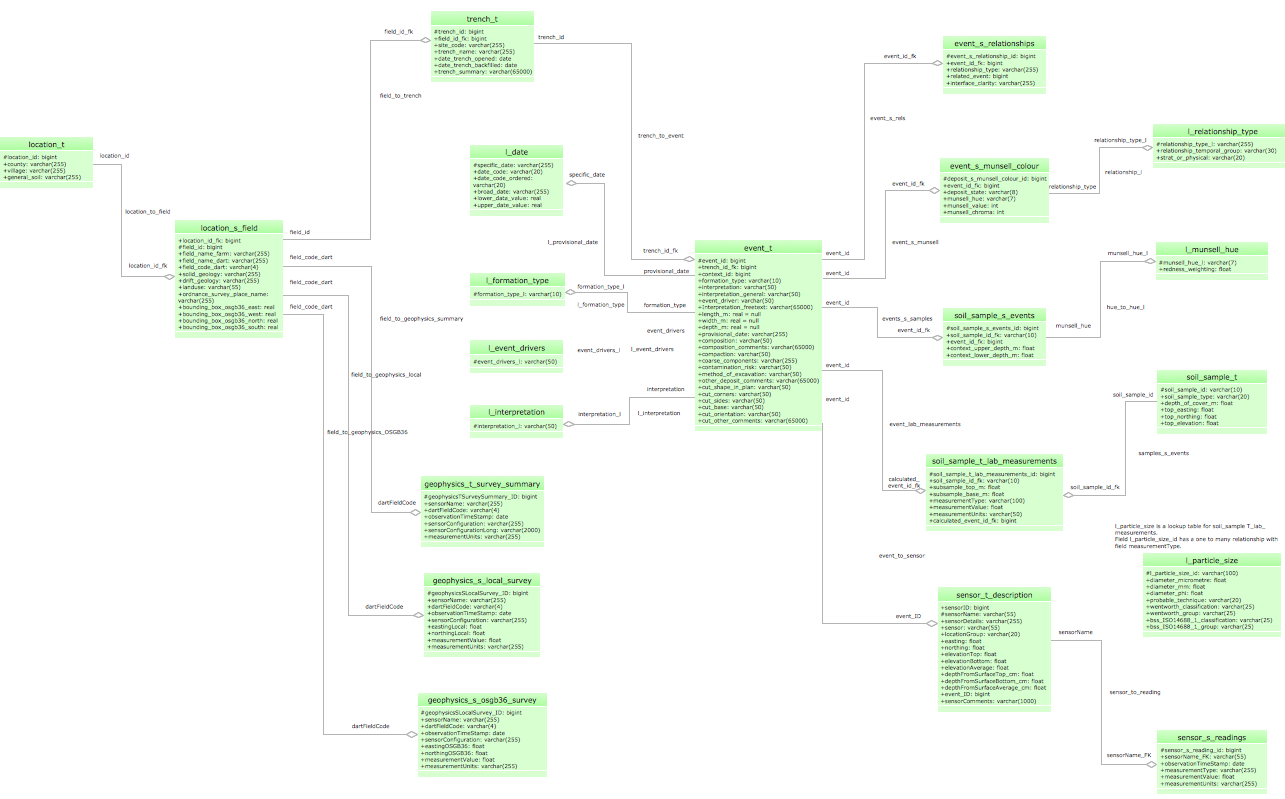
\includegraphics[width=\textwidth]{complex_model}
  \caption{Complex model in UML}
  \label{fig:model}
\end{figure}


Then with the simulation of these systems, we can imagine that we are able to find all possible states of our
system. So we know that if we are not in a valid state of the system, the system was potentially hacked.

\section{Position of my project}

So for my project, I guess I have all possible states for my system and I will check these possible states with the
current status of the system. To do so, I have to find the state of applications and the state of the network, and
analyze them.

I choose to use an IDS to have the status of the network. In fact, an IDS can raise alert when there is particular
message, so I will raise event when I sniff particular message. To have a status of an application, I choose to
implement probe in applications, or if it is possible use the log of these applications. Then, the SIEM will
correlate all these messages and alerts to find the status of our system and it will compare it with all previous
possible status.


The figure \ref{fig:model_project} represent the position of our project.

\begin{figure}[h]
  \centering
  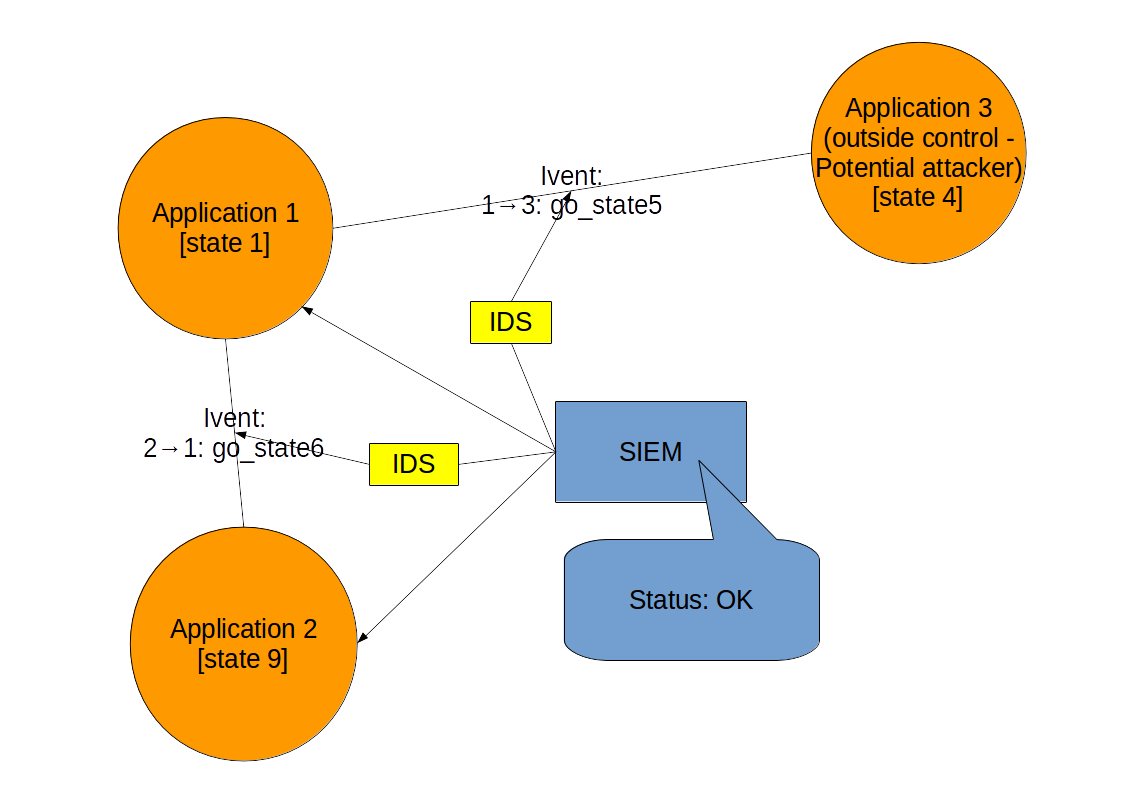
\includegraphics[width=\textwidth]{model_project}
  \caption{Position of my project}
  \label{fig:model_project}
\end{figure}




%%% Local Variables:
%%% mode: latex
%%% TeX-master: "../rapport_de_base"
%%% End:

  
\chapter{Technical choice}
\label{chap:choice}

\section{Application created for test}

As it was explain before, I have to protect a specific application. To do my tests, and prove the concept of my
work, I choose to create a simple application. I plan to add some security issue to be more realistic.~\\


This application have three states, and two part. Firstly, there is an admin interface which contain the state
admin. This interface is connected on the port 9000. Only one specific known computer can access to this interface.
Of course, the aim of attackers is to arrive in this state.

Then there is the main application. It is connected to the port 9124, and everybody can connect to it. There is two
state ping and pong. If the application is in the state ping and the user send <<topong>> the application go to state
pong, and if the application is in the state pong and the user send <<toping>> the application go to the state ping.
There is also an unknown backdoor, if the user is in the state ping for the third time and he send <<admin>>, the
application go to the admin interface.

The figure \ref{fig:appli} represent a model of our application.


\begin{figure}[!h]
  \centering
  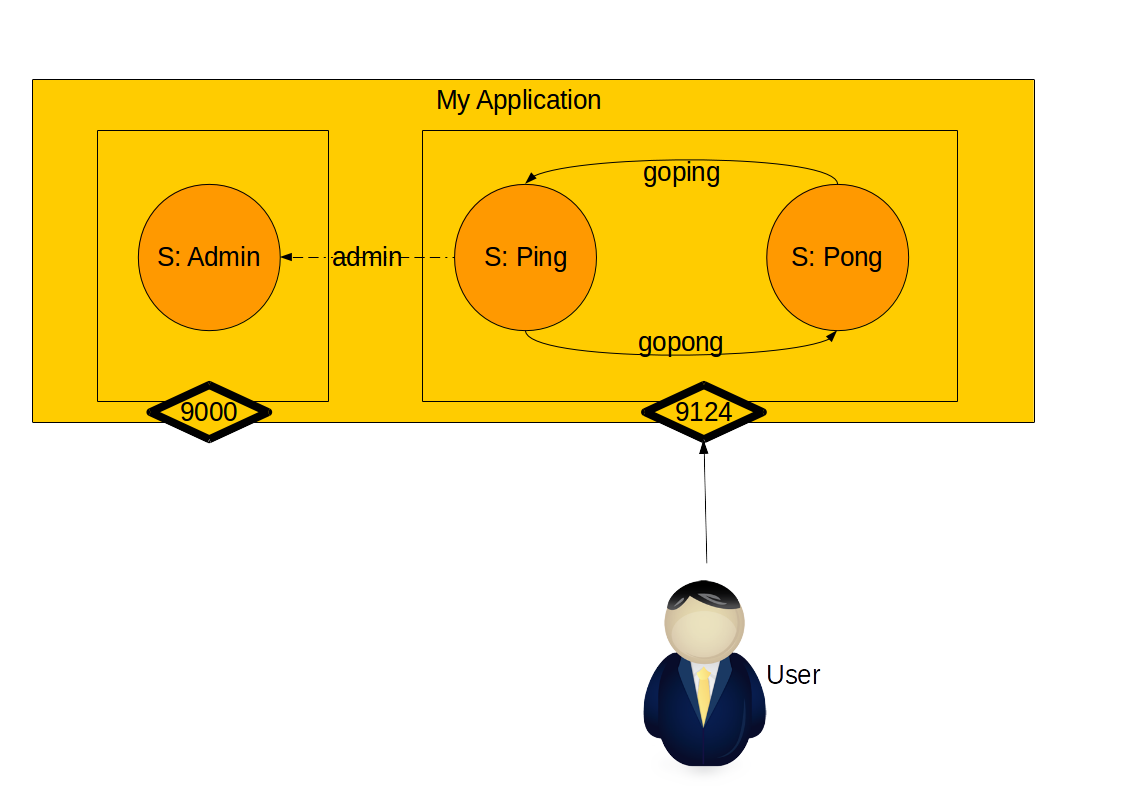
\includegraphics[width=0.9\textwidth]{appli}
  \caption{Model of the application}
  \label{fig:appli}
\end{figure}

\section{IDS}

To monitor the network between my applications, I have to install an IDS. In this project, my IDS only need to check
network packets and send alert when it detects some pattern. So I choose to use a IDS which use a misuse detection.

Moreover, my IDS only need to raise alert and save them. It is possible to find on the market of open source
software many IDS which do that. So I choose one of the most popular open source IDS, SELKS.

\section{SIEM}

Then, for the SIEM I had to made a choice: use an open source solution of SIEM, or implement my own solution. The
table \ref{tab:preludevssiem} lists advantages and drawback of the two solutions.

\begin{table}[h]
  \centering
  \begin{tabularx}{1.0\linewidth}[h]{|X|X|}
    \hline
    \multicolumn{2}{|>{\centering\hsize=2\hsize}X|}{\textbf{Prelude}}\\
    \hline
    Advantages & Drawbacks \\
    \hline
    Already implemented & Need to connect it to SELKS \\
    \hline
    More modular  & Not adapted to my problem \\
    \hline
               & Need to configure it \\
    \hline
               & Heavy solution \\


    %%%%%%%%%%%%%%%%%%%%%%%%%%%%%%%%%%%%%%%%
    \hline
    \hline
    \multicolumn{2}{|>{\centering\hsize=2\hsize}X|}{\textbf{My SIEM}}\\
    \hline
    Advantages & Drawbacks \\
    \hline
    Well adapted for my problem & Need time to implement it \\
    \hline
    Less heavy & Only adapted for my problem\\

    \hline

  \end{tabularx}
  \caption{Prelude vs my SIEM}
  \label{tab:preludevssiem}
\end{table}

For all the reasons cited on the previous table, I choose to implement my own SIEM.


%%% Local Variables:
%%% mode: latex
%%% TeX-master: "../rapport_de_base"
%%% End:

  
\chapter{Position of the Project}
\label{chap:project}


\section{Resume}

\section{Technical choice}


\section{Forecasting organization}

\subsection{Kanban}

To realize this project, I decided to use some tools to arrange my work. First
of all, I decided to use a agile technique of management which name Kanban.~\\

\definition{Kanban}{Kanban is a new technique for managing a software
  development process in a highly efficient way. Kanban underpins Toyota's
  "just-in-time" (JIT) production system. kanban system consists of a big board
  on the wall with cards or sticky notes placed in columns with numbers at the
  top \cite{peterson:kanban}}


Kanban is an inventory-control system to control the supply chain. It use a
board with columns. Each columns represent a status, for example: to do, doing,
done. In each column we put <<notes>> which represent a task. Moreover, each
column have a maximum number of notes authorized.

%%%%%%%%%%%%%%%%%%%%%%%%%%%%%%%%%%%%%%%%%%%%%%%%%%%%%%%%%%%%%%%%%%%%%%%%%%%%
%% TODO: Rajouter une image
%%%%%%%%%%%%%%%%%%%%%%%%%%%%%%%%%%%%%%%%%%%%%%%%%%%%%%%%%%%%%%%%%%%%%%%%%%%%


Limiting the amount of task, at each step in the process, prevents
overproduction and revels bottlenecks dynamically. In fact, with this technique
it is possible to have a better overview of the project and control it dynamically.
~\\

For this project, I use Kanboard\cite{guillot:kanboard} self-hosted on my own server.\footnote{\url{https://mic-rigaud.fr/kanboard/?controller=BoardViewController&action=readonly&token=10ea65eca908023dbcd8bc8dce75791c7a14d67912627dafaa5b71033222}}


\subsection{Github}

To realize this project, I also decided to use Git and Github as Git server. ~\\

\definition{Git}{Git is a version control system for tracking changes in
  computer files and coordinating work on those files among multiple people.}

Git permit for me to control version of my work and have a real showcase of my
work for my tutor. The figure \ref{fig:github} is a screenshot of my Github
server.

\begin{figure}[h]
  \centering
  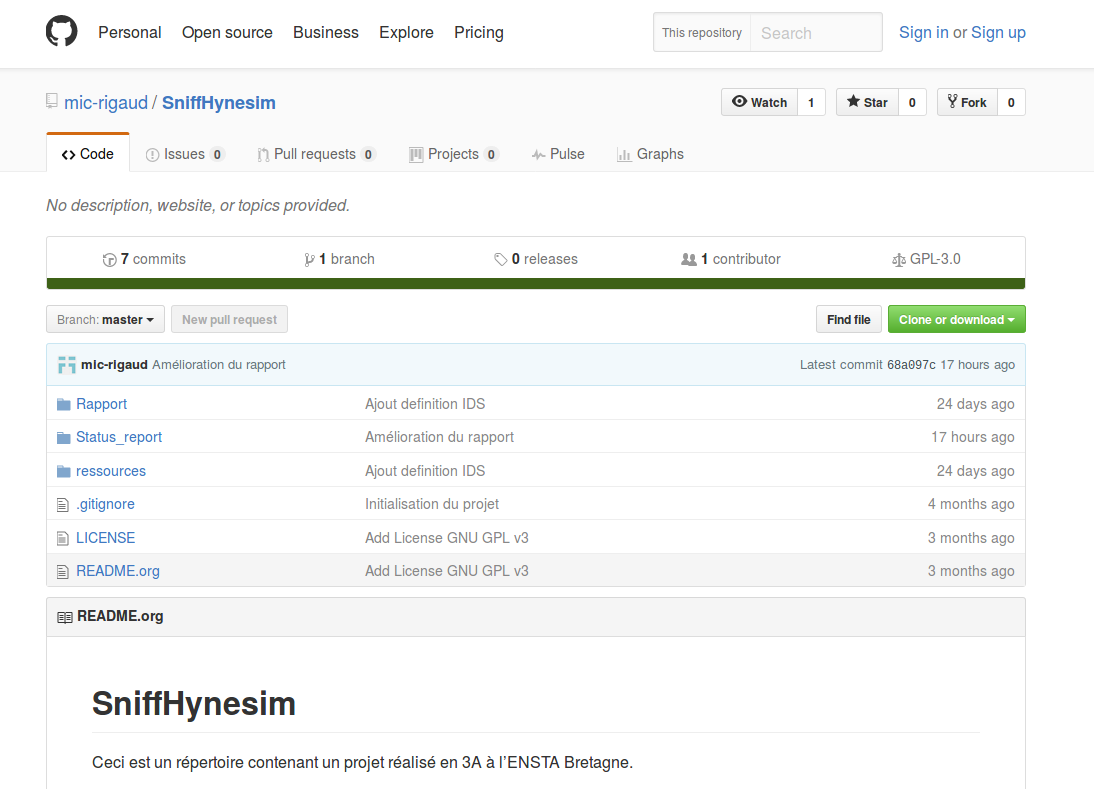
\includegraphics[width=\textwidth]{github}
  \caption{Github server}
  \label{fig:github}
\end{figure}

%%%%%%%%%%%%%%%%%%%%%%%%%%%%%%%%%%%%%%%%%%%%%%%%%%%%%%%%%%%%%%%%%%%%%%%%%%%%
%% TODO: Rajouter une image
%%%%%%%%%%%%%%%%%%%%%%%%%%%%%%%%%%%%%%%%%%%%%%%%%%%%%%%%%%%%%%%%%%%%%%%%%%%%



%%% Local Variables:
%%% mode: latex
%%% TeX-master: "../rapport_de_base"
%%% End:


\part{Technical study}
  
\chapter{Installation}

\section{Hynesim}

\subsection{Requirement}

To use Hynesim, Justin and I had to install the open source version of Hynesim server. To do so, M Champeau give us
a computer with 16G of RAM. I installed Debian 8 on this machine. Them I installed the hynesim server with the
basics networks equipment. I follow the instructions write on the Hynesim web-page.

Then, Justin configure Hynesim to be accessible with the client. I will not detail this part, if you want more
information you can read his report.


\subsection{Import of virtual machines}

Hynesim works with many virtual software as qemu, virtualbox, and vmware. For this project I use qemu because it is
the most suitable for hynesim. To create virtual computer on hynesim, I firstly created the machine on virtualbox,
then I converted it to a qemu virtual machine and to finish I import this machine to hynesim.

Hynesim is also provided with some virtual equipment: a switch, and an inter topology link.

An important detail, on the hynesim network machines haven't access to the internet. So I had to do update, and
install before they are imported.

I created the left part of the network represented on the figure \ref{fig:network}.


\begin{figure}[h]
  \centering
  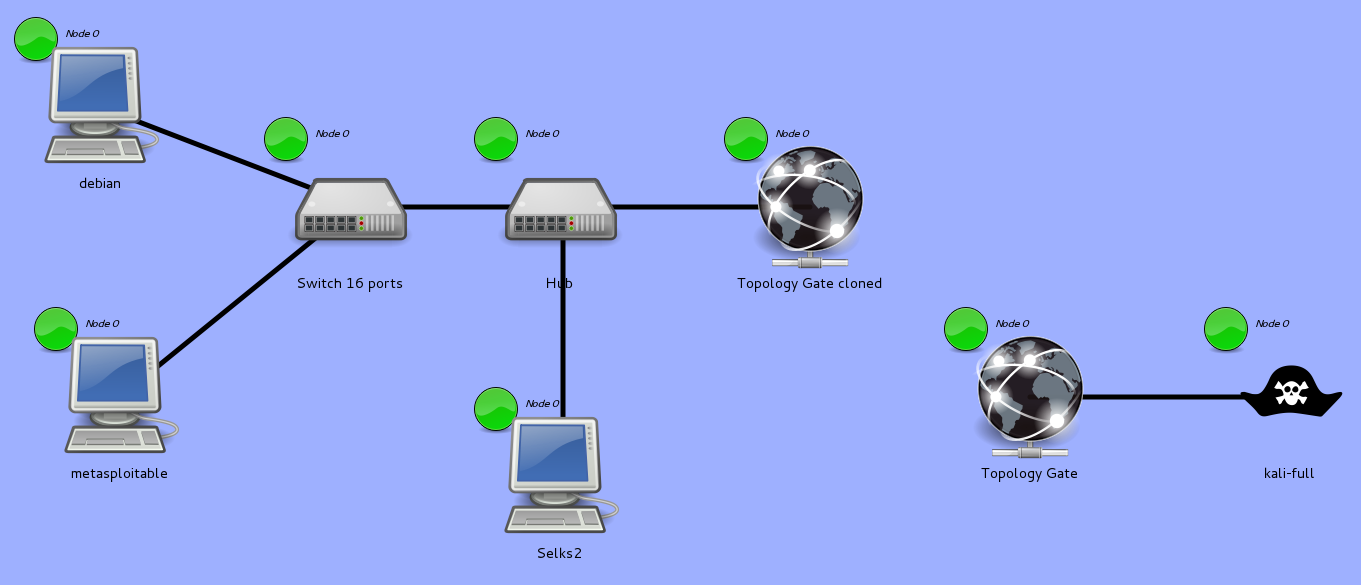
\includegraphics[width=\textwidth]{network_infra}
  \caption{Network infrastructure}
  \label{fig:network}
\end{figure}

\section{Selks}

As it was explain on the previous section, before importing the machine I had to create an virtual machine. To do
so, I use an ISO available on the Stamus web page \cite{stamusnetworks:_selks} and I create a virtual machine with
it. Then, before it was imported, I have set up important libraries for the realization of the SIEM\footnote{More
  information on the chapter \ref{sec:SIEM}}.

The ISO is a key in hand version. So Suricata, Elasticsearch, Logstash, Kibana, Scirius, and Evebox are already
installed and connected.\footnote{For more information you can can read the annex \ref{chap:selks}} However, I had
to configure some particularity and take in charge the system.

The only particularity that I have to configure during the installation was the network. In fact, on the hynesim
network there is no DHCP, so I had to configure by hand the IP of the machines. Moreover, I had to configure on
Suricata the private address domain. In fact, Suricata doesn't pay so much attention to networks packets from the
private network.

Then, I tested my IDS with basic attacks\footnote{These attacks were achieve by Justin Bouroux}. The can see on the
figure \ref{fig:evebox} the evebox interface which permit to visualize alerts raised by Suricata.

\begin{figure}[h]
  \centering
  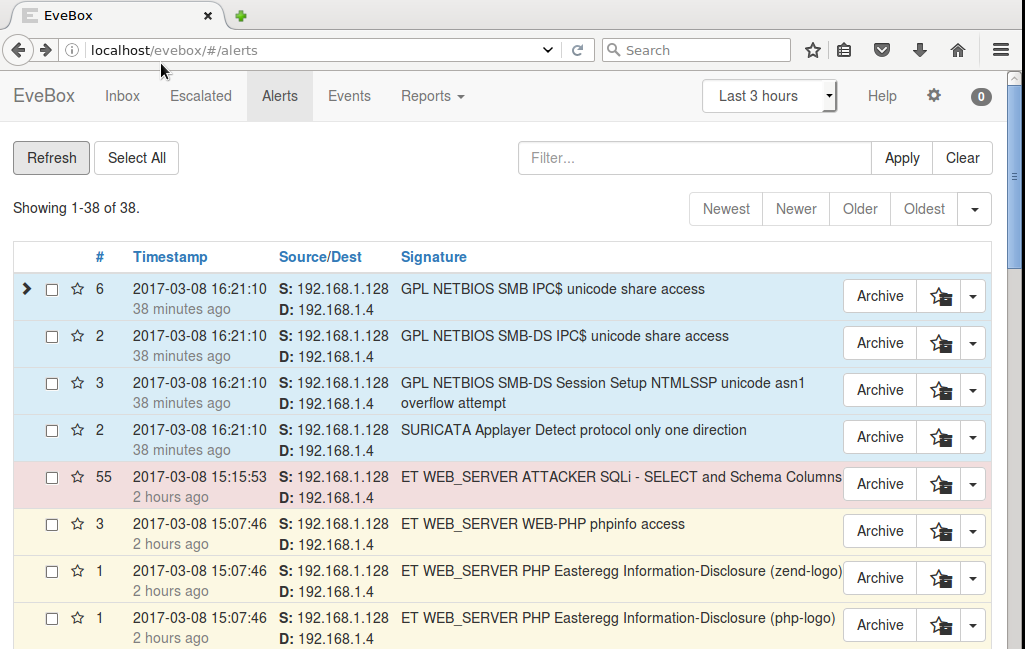
\includegraphics[width=\textwidth]{evebox}
  \caption{Example of alerts}
  \label{fig:evebox}
\end{figure}


%%% Local Variables:
%%% mode: latex
%%% TeX-master: "../rapport_de_base"
%%% End:

  
\chapter{Implementation}

In this chapter, I will explain how I implemented my solution.

\section{Application}

First of all, I implemented the application for the tests. I choose to implement this application in python and it
is hosted on the computer named Dedian (cf figure \ref{fig:network}). As it was explain in the chapter
\ref{chap:choice}, this application has three state: Ping, Pong and Admin.

Considering I have to implement the defense of this application, I have to delimit the sensitive space. It is
obvious for this application, the sensitive state is the admin state. So I have to send many event when the user
try to access to the admin interface. In this way I could know if somebody try without success to access to the
admin interface, this person is doubtless an attacker.

To raise event, I send messages to a particular Logstask instance which is on SELKS. These messages contain the
time and the state of the application. I will explain after, how the Logstash instance work.

\begin{table}[h]
  \centering
  \begin{tabularx}{1.0\linewidth}{|X|X|}
    \hline
    Hosted&Debian\\
    \hline
    Language & Python \\
    \hline
    States & Ping, Pong, Admin \\
    \hline
    Sensitive state & Admin \\
    \hline
    Port open & 9124, 9000\\
    \hline
    Outdoor communication & Selks to port 5000 \\
    \hline
    Port 9124 accept communication from & Everybody \\
    \hline
    Port 9000 accept communication from & Metasploitable only\\
    \hline
  \end{tabularx}
  \caption{Features of the application}
  \label{tab:carac}
\end{table}


\section{Probe}

\subsection{Network probe}

I already explain that I use SELKS as IDS, but I had to configure it to adapt it to my application. So I had rules
on the Suricata ruleset. To add rules, I use the scirius interface which permit to administrate suricata's ruleset.
I added the next rules:

\begin{lstlisting}[language=suricata]
  alert tcp any any -> any 9124 (msg:"Action goping"; \
  content:"goping"; sid:501; rev:5000;)

  alert tcp any any -> any 9124 (msg:"Action gopong"; \
  content:"gopong"; sid:502; rev:5001;)

  alert tcp any any -> any 9000 (msg:"Connexion vers l interface admin"; \
  flow:established,to_server sid:504; rev:5002;)
\end{lstlisting}




\subsection{Application probe}

As it was explain before, to have the status of the application, it sends to Logstash its status. Then, Logstash
filter these messages and write them on the Elasticsearch data base.

On the SELKS computer, there is a Logstash implemented with a filter adapted for Suricata but not for our
application. So I write a filter to Logstash adapted for this application, and I run a new instance of Logstash
with this configuration on SELKS. By this way, both instance of Logstash do their job without interaction.

The filter implemented, convert plain text message send by my application as json event readable by Elasticsearch.
Moreover, the filter add some tag on this events facilitate the research on the data base. These tags are added on the
label <<alert\_signature\_id>>.

\begin{figure}[h]
  \centering
  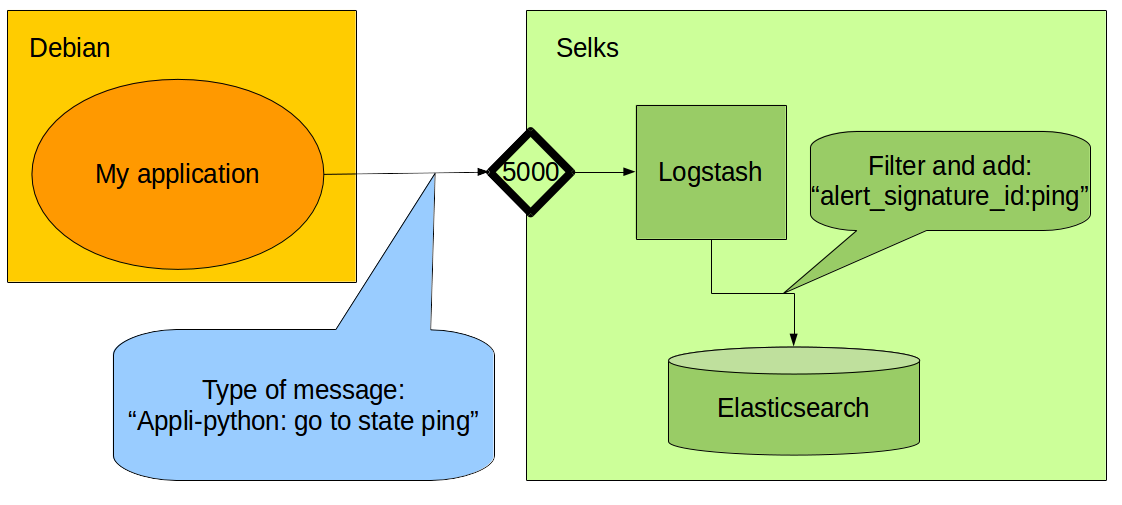
\includegraphics[width=\textwidth]{traitement_donnes}
  \caption{Data processing}
  \label{fig:dataprocessing}
\end{figure}


\section{SIEM}
\label{sec:SIEM}

I also achieve to implement a SIEM. To do so, I used the <<elasticsearch>> library for python. With it I can make
request to the data base easily. I collect the last events, I refresh the interface with these information, and
analyze its. After analysis, I am able to say if the application is under attack.

The figure \ref{fig:mysiem} represent the interface of the SIEM implemented.


\begin{figure}[h]
  \centering
  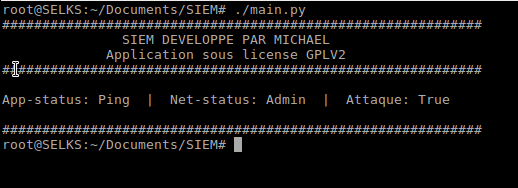
\includegraphics[width=0.7\textwidth]{siem_interface}
  \caption{My siem interface}
  \label{fig:mysiem}
\end{figure}

\newpage
\section{Summary}

The next figure represents a summary of the infrastructure of our system.

\begin{figure}[h]
  \centering
  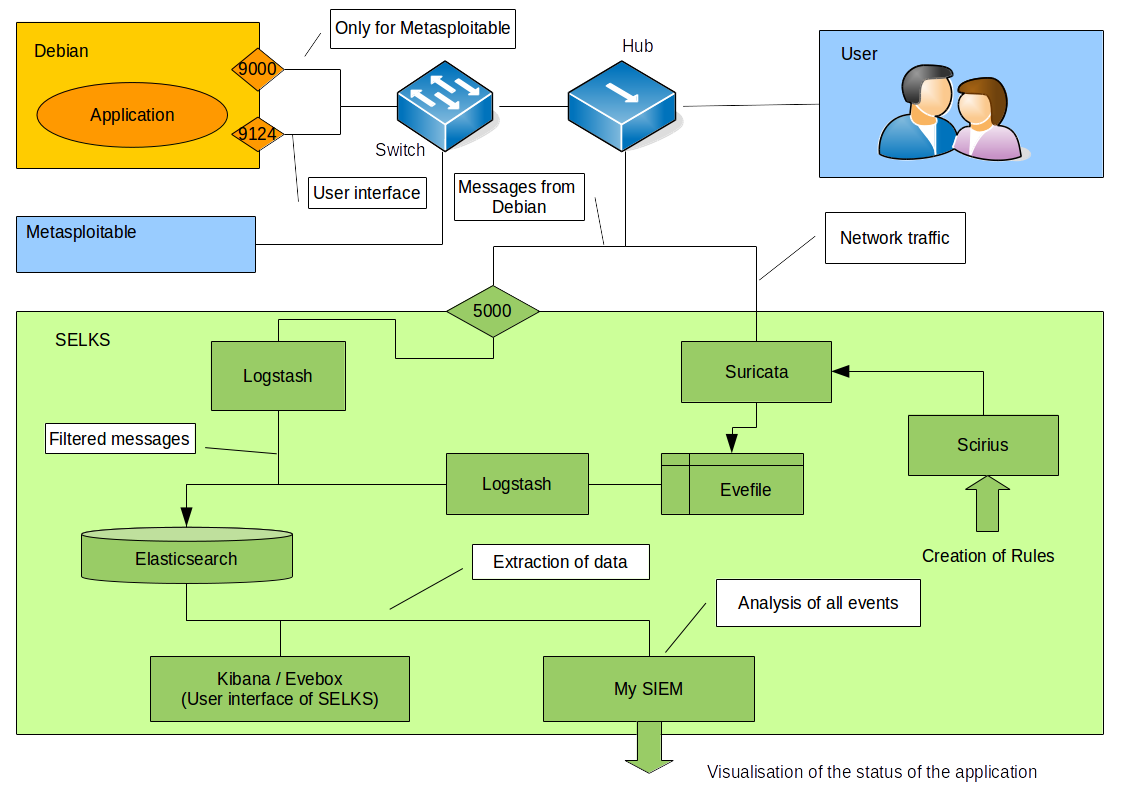
\includegraphics[width=\textwidth]{summary}
  \caption{Summary of the situation}
  \label{fig:summ}
\end{figure}

%%% Local Variables:
%%% mode: latex
%%% TeX-master: "../rapport_de_base"
%%% End:

  
\chapter{Analysis of results}
\label{chap:analysis}


\section{Results}

In the system represented before, I represented the cyber defense. On the same system, Justin Bouroux achieved
attacks and tried to penetrate the system. Of course, it was designed to have some security issues, but the most
important for my system is the detection of its attacks. In fact, all system have security issue even the most
secure\footnote{A minimum of <<zero day>>}, but if we can detect an intrusion we are able to ensure the service. If
you want more information about attacks carried out, you can read the Justin's report.
~\\

Firstly we can notice that my system was able to detect the scan of ports. In fact, when Justin try to scan all the
ports of the Debian, Suricata raised some warnings. This warnings represent a possible attacks. It is very important
to detect that because it is often the synonym that someone want to attack your system.

\begin{figure}[h]
  \centering
  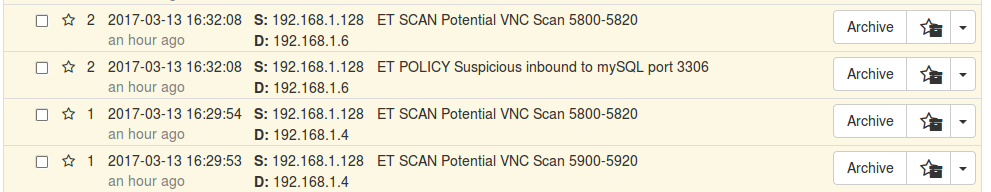
\includegraphics[width=\textwidth]{scan}
  \caption{Events raised during the scan}
  \label{fig:scan}
\end{figure}



Then, he has tested the application. It is possible to see the events ping and pong on the network, and the events
send by the application. The SIEM implemented resume these changes of states.

\begin{figure}[h]
  \centering
  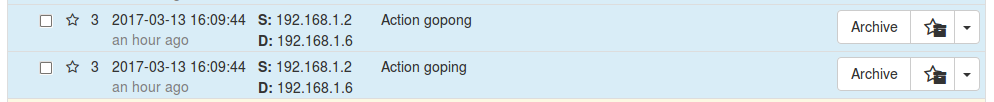
\includegraphics[width=\textwidth]{goping_gopong}
  \caption{Events goping and gopong}
  \label{fig:gopong}
\end{figure}


Justin, also try to access to the admin interface with the combination of <<to\_ping>>, <<to\_pong>>, and
<<admin>>. It is possible to notice, that my system of detection is able to detect this attack. On the network the
attack seems invisible because he isn't logged in the port 9000, but the application send the event <<appli-python:
go to admin state>>. So, the system is under attack.

\begin{figure}[h]
  \centering
  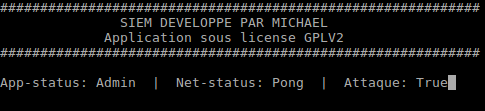
\includegraphics[width=0.7\textwidth]{admin_fuz}
  \caption{SIEM interface}
  \label{fig:fuzz}
\end{figure}


And to finish, Justin hacked the metasploitable computer to have access to the admin interface on the port 9000.
After his attack, my system of detection raise a lot of alert. Firstly, because the IDS has detected his attack
against the metasploitable. Secondly, because the application has raised event when he arrived on the admin
interface. So, I am able to identify his attack against the metasploitable and connect it to the access of the
admin interface.


\begin{figure}[h]
  \centering
  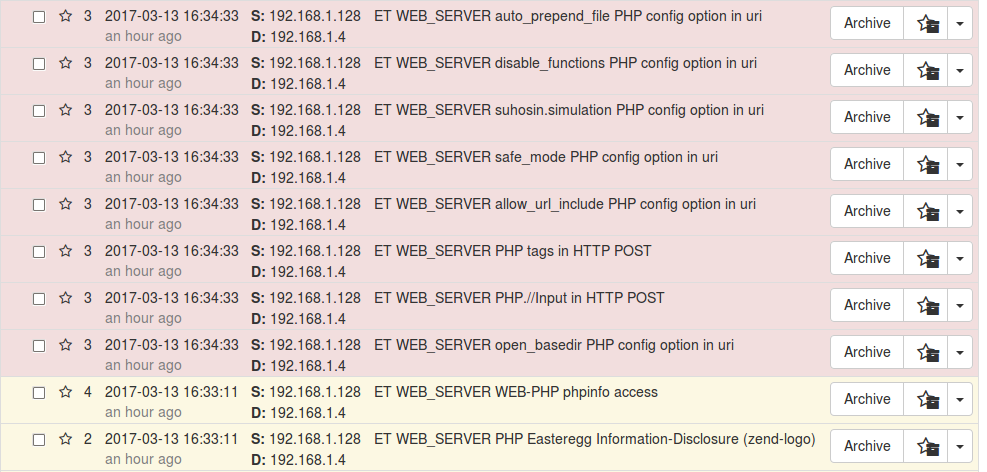
\includegraphics[width=\textwidth]{attacks}
  \caption{Alerts during metasploitable attacks}
  \label{fig:attcks}
\end{figure}

A demonstration video will be presented during the presentation.


\section{Way of improve}

To summarize, during this test phase I was able to detect all attacks. However, I had some issue. In fact, the
Suricata IDS sometimes raises event later. Sometimes 5 minutes after the real event. It is not a problem for a
normal IDS, but for our utilization it is. We want to know the states of our system without delay to analyze them.
Even if I think the problem can be solved with computer more efficient, it is a real issue.

Moreover, I didn't protect my detector system because the lack of time, so it is possible to attack it. For
example, it is possible to send false messages to the SIEM to hide attacks. It would be necessary to add an
authenticity on the messages send by the application to the SIEM.




%%% Local Variables:
%%% mode: latex
%%% TeX-master: "../rapport_de_base"
%%% End:




%%%% CONCLUSION %%%%%%%%%

\chapter*{Conclusion}
\addcontentsline{toc}{chapter}{Conclusion}


After this study, I got to implement a system of detection. But because of the lack of time, I achieved a simple
system, which is based on SELKS and on a SIEM implemented by me. This system is adapted to the application used for
the tests but it needs some improvements to be adapted for other applications.

We can also notice that my system of detection can also be attacked which has not been envisaged in this study.

To conclude, I achieve a simple system of detection which need some improvements. However, this system prove that
it is possible to retrieve all the states of an observed system. And if we could model this observed system, we
would be able to extract all the possible states of the system via model checking. Then, we could compare this
possible states with the current state of the system to detect attacks.

So it is a prove of contest of the possibility to use model checking to implement the security rules of an
application.




\newpage

%%%% ANNEXE %%%%%%%%%%%%

\part*{Annex}
\appendix
\nocite{*}

\chapter{SELKS}
\label{chap:selks}

\definition{SELKS}{SELKS is a free and open source Debian (with LXDE X-window manager) based IDS/IPS platform released under GPLv3 from Stamus Networks (https://www.stamus-networks.com/).\cite{stamusnetworks:_selks}~\\

The SELKS ISO is both Live and Installable ISO in one. Once installed it is ready to use out of the box solution. ~\\

SELKS is comprised of the following major components:
\begin{itemize}[itemsep=0pt]
\item[\textbf{S}] Suricata IDPS - http://suricata-ids.org/
\item[\textbf{E}] Elasticsearch - http://www.elasticsearch.org/overview/
\item[\textbf{L}] Logstash - http://www.elasticsearch.org/overview/
\item[\textbf{K}] Kibana - http://www.elasticsearch.org/overview/
\item[\textbf{S}] Scirius - https://github.com/StamusNetworks/scirius
\end{itemize}
}

So SELKS is an OS which contain the Suricata IDS. It also contain Elasticsearch to analyze alerts, Logstash to
analyze log, Kibana to have overview of alerts, and Scirius to add rules.

You can see on figure \ref{fig:kibana}, an example of the interface of kibana which give an overview of the alerts.
This image was extract from the Twitter of Stamus Networks.



\begin{figure}
  \centering
  
\includegraphics[width=\textwidth]{selks_desktop}
  \caption{screenshot of SELKS desktop}
  \label{fig:selks}
\end{figure}

\begin{figure}[h]
  \centering
  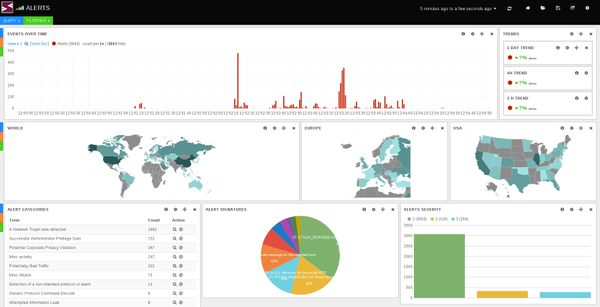
\includegraphics[width=\textwidth]{kibana}
  \caption{Kibana interface}
  \label{fig:kibana}
\end{figure}


%%% Local Variables:
%%% mode: latex
%%% TeX-master: "../rapport_de_base"
%%% End:

\newpage
 \listoffigures
 \printindex
 \bibliographystyle{plain}
  \bibliography{biblio}

\end{document}
%%%%%%%%%%%%%%%%% FIN DU DOCUMENT
%%% Local Variables:
%%% mode: latex
%%% TeX-master: t
%%% End:
